\documentclass[a4paper]{article}
\usepackage[affil-it]{authblk}
\usepackage[backend=bibtex,style=numeric]{biblatex}
\usepackage{geometry}
\usepackage{amsmath}
\usepackage{float, caption}
\usepackage{graphicx}
\geometry{margin=1.5cm, vmargin={0pt,1cm}}
\setlength{\topmargin}{-1cm}
\setlength{\paperheight}{29.7cm}
\setlength{\textheight}{25.3cm}

\addbibresource{citation.bib}

\begin{document}
% =================================================
\title{Numerical Analysis homework \# 4}

\author{Guang Zhang 3230105121
  \thanks{Electronic address: \texttt{zhuiguang49@foxmail.com}}}
\affil{(Information and Computing Science, Class XJ2301), Zhejiang University }

\date{finish time: \today}

\maketitle






% ============================================
\section*{I. Question I}

We just need to consecutively divide $477$ by $2$ and record its remainder until the remainder is $0$, then concatenate
the remainder bakwards. Thus, we can obtain that $(477)_{10}=(111011101)_2=(1.11011101)_2\times 2^8$

\section*{II. Question II}

We can just follow Algorithm 4.8, multiply the fraction $\frac{3}{5}$ by $2$, if the integer part is less than $1$, we record $1$; else we record $0$. And repeat the algorithm with its fraction part.
Thus, we can obtain that $(\frac{3}{5})_{10}=(0.\overline{1001})_{2}=(1.0011001\cdots)_2\times 2^{-1}$


\section*{III. Question III}

It is easy to obtain that $x=\beta^e=1\times \beta^e$, while $x_R=x+\beta^{1-p} \beta^e$, so we have $x_R-x=\beta^{1-p+e}$. while
$x_L=(\beta-\beta^{1-p})\beta^{e-1}$, so we have $x-x_L=\beta^{1-p} \beta^{e-1}=\beta^{e-p}$. Then we can obtain that $(x_R-x)=\beta(x-x_L)$


\section*{IV. Question IV}

From Question II, we have $x=(0.\overline{1001})_2=(1.0011001\cdots)_2\times2^{-1}$, while $x_{R}=(1.0011001\cdots 1010)_2\times 2^{-1},x_L=(1.0011001\cdots1001)_2\times 2^{-1}$, then we can compute $x_R-x$ and $x-x_L$.\newline
We have $x-x_L=(0.0\cdots1001\cdots)_2\times 2^{-1}=(1.0011\cdots)_2\times 2^{-25}=\frac{3}{5}\times 2^{-24}$, and $x_R-x=(x_R-x_L)-(x-x_L)=(0.0\cdots01)_2\times 2^{-1}-\frac{3}{5}\times 2^{-24}=(1-\frac{3}{5})\times 10^{-24}=\frac{2}{5}\times 2^{-24}$.\newline
Therefore, we have $x_R-x<x-x_L$, which means that $fl(x)=x_R=(1.001001\cdots1010)_2\times 2^{-1}$, and the relative roundoff error is $E_r=|\frac{x_R-x}{x}|=\frac{2}{3}\times 2^{-24}$

\section*{V. Question V}

If we round to the nearest, the maximum error is at most half the distance between two adjacent floating point numbers, so in that case $\epsilon_u=\frac{1}{2}\epsilon_M$. However, if we drop excess bits, the caculated value is always rounded down to the nearest representable number. In the
worst case, the number may be infinitely close to the next larger FPN, then the error can span the entire distance between two adjacent numbers. Therefore, the unit roundoff $\epsilon_u$ would become equal to the machine precision, that is to say $\epsilon_u=\epsilon_M=\beta^{1-p}=2^{-23}$

\section*{VI. Question VI}

By Theorem 4.49, we need to compute $1-\frac{\cos x}{1}$ when $x=\frac{1}{4}$, that is, compute $1-\cos \frac{1}{4}$.
By calculator, we can obtain that $1-\cos(\frac{1}{4})\approx0.0310876$, while $2^{-6}\le0.0310876\leq 2^{-5}$, so by theorem 4.49 we can obtain that $1-\cos\frac{1}{4}$ loses at least $5$ bits and at most $6$ bits of precision.

\section*{VII. Question VII}

To avoid catastrophic cancellation cause by subtraction, we can avoid using subtraction to compute $1-\cos x$, in other words, using other operations by transforming the formula.

\subsection*{Method 1 Half angle formula}

Through the \textbf{Half Angle Formual}, we have $\cos x = 1-2\sin^2\frac{x}{2}$, then $1-\cos x$ can be transformed into $2\sin^2\frac{x}{2}$, which can avoid subtraction.

\subsection*{Method 2 Difference of squares formula}

We can multiply both the numerator and denominator by $(1+\cos x)$ simultaneously, then $1-\cos x$ can be turned into $\frac{(1-\cos x)(1+\cos x)}{1+\cos x}=\frac{\sin^2 x}{1+\cos x}$, which also aviod subtraction.

\section*{VIII. Question VIII}

\subsection*{VIII.a $(x-1)^{\alpha}$}

Denote $f(x)=(x-1)^{\alpha}$, then the deriative of $f(x)$ is $\alpha(x-1)^{\alpha-1}$, and through Definition 4.59, we can obtain that the condition number $C=|\frac{xf'(x)}{f(x)}|=\big|\frac{\alpha x}{x-1}\big|,x\neq 1$, and it is easy to know that
$C$ is large when $x\to 1$.

\subsection*{VIII.b $\ln x$}

Denote $f(x)=\ln x(x>0)$, then the deriative of $f(x)$, $f'(x)$ would be $f'(x)=\frac{1}{x}(x>0)$, then the condition number $C=|\frac{xf'(x)}{f(x)}|=\big|\frac{1}{\ln x}\big|(x>0,x\neq 1)$, and it is easy to know that $C$ is large when $x\to 1$.

\subsection*{VIII.c $e^{x}$}

Denote $f(x)=e^{x}$, then the deriative  of $f(x)$, $f'(x)$ would be $f'(x)=e^x$, then the condition number $C=|\frac{xf'(x)}{f(x)}|=\big|\frac{xe^x}{e^x}\big|=|x|$. It is easy to know that $C$ is large when $x\to \infty$.

\subsection*{VIII.d $\arccos x$}

Denote $f(x)=\arccos x$, then the deriative of $f(x)$, $f'(x)$ would be $f'(x)=-\frac{1}{\sqrt{1-x^2}},x\in(-1,1)$, then the condition number $C=|\frac{xf'(x)}{x}|=\big|\frac{x}{\sqrt{1-x^2}\arccos x}\big|,x\in(-1,1)$, $\sqrt{1-x^2}\to 0$ when $x\to -1$ or $x\to 1$, and $\arccos x$ is bounded when $x\in(-1,1)$, so $C$ 
is large when $x\to -1$ or $x\to 1$.

\section*{IX. Question IX}

\subsection*{IX.a}

The deriative of $f(x)$ is $f'(x)=e^{-x}$, so we can obtain that $cond_f(x)=|\frac{xf'(x)}{f(x)}|=\frac{xe^{-x}}{1-e^{-x}},x\in[0,1]$, then we need to prove $\frac{xe^{-x}}{1-e^{-x}}\leq 1\iff e^{-x}(x+1)\leq 1$.
It is acknowledged that $e^x\geq x+1$ holds for all $x\in R$, then we can obtain that $e^{-x}\leq \frac{1}{x+1}$ for all $x\geq 0$, then we have $e^{-x}(x+1)\leq 1$ holds for all $x\in[0,1]$, so $cond_f(x)\leq 1$ for $x\in[0,1]$ is verified.

\subsection*{IX.b}

Denote the algorithm $A$ as $f_A(x)$, with an input $x$, the computer actually implements two steps:
\begin{enumerate}
  \item \textbf{compute the exponent:} $fl(e^{-x})=(e^{-x})(1+\delta_1)$
  \item \textbf{compute the subtraction:} $fl(1-e^{-x})=(1-fl(e^{-x}))(1+\delta_2)=[1-e^{-x}(1+\delta_1)](1+\delta_2)$
\end{enumerate}
where $|\delta_1|,|\delta_2|\leq \epsilon_u$, then we can obtain that $f_A(x)=1+\delta_2-(1+\delta_1+\delta_2+\delta_1\delta_2)e^{-x}\approx 1+\delta_2-(1+\delta_1+\delta_2)e^{-x}$, then we have
\begin{equation}
  f_A(x)=f(x)+\delta_2f(x)-\delta_1e^{-x}
\end{equation}
then the relative error would be 
\begin{equation}
  \big|\frac{f_A(x)-f(x)}{f(x)}\big|=\big|\frac{\delta_2f(x)-\delta_1e^{-x}}{f(x)}\big|=\big|\frac{e^{-x}}{1-e^{-x}}\delta_1-\delta_2\big|\leq \big|\frac{e^{-x}}{1-e^{-x}}\big|\big|\delta_1\big|+\big|\delta_2\big|
\end{equation}
While $|\delta_1|,|\delta_2|\leq \epsilon_u$, we can obtain that
\begin{equation}
  \big|\frac{f_A(x)-f(x)}{f(x)}\big|\leq (\frac{e^{-x}+1-e^{-x}}{1-e^{-x}})\epsilon_u=\frac{1}{1-e^{-x}}\epsilon_u
\end{equation}
Then $\varphi(x)$ in Theorem 4.78 would be $\frac{1}{1-e^{-x}}$, thus we have $cond_A(x)$ satisfies
\begin{equation}
  cond_A(x)\leq \frac{\varphi(x)}{cond_f(x)}=\frac{\frac{1}{1-e^{-x}}}{\frac{xe^{-x}}{1-e^{-x}}}=\frac{e^x}{x} \qquad x\in[0,1]
\end{equation}

\subsection*{IX.c}

The picture of $cond_f(x)$ and the estimated upper bound of $cond_A(x)$ is as follows:

\begin{figure}[H]
  \centering
  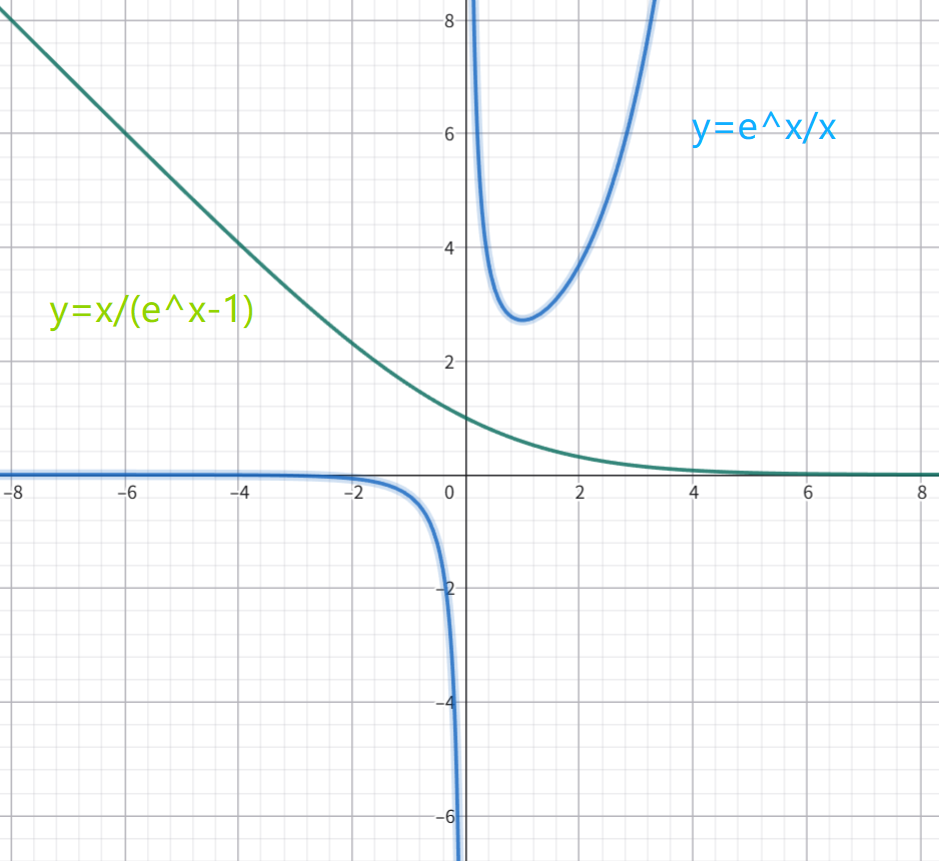
\includegraphics[width=0.8\textwidth]{Picture1.png} 
  \caption{The picture of $cond_f(x)$ and the estimated upper bound of $cond_A(x)$.}
\end{figure}

The blue line in the picture is the estimated upper bound of $cond_A(x)$, while the green line in the picture is $cond_f(x)$. As we have obtained in IX.a, $cond_f(x)\leq 1$ holds
for all $x\in[0,1]$, which means the problem itself is well-conditioned. However, when $x\to 0$, we could notice that the upper bound of $cond_A(x)\to \infty$, which means that the algorithm(substract directly) is not stable, which actually is catastrophic cancellation.
To avoid catastrophic cancellation, we should avoid direct subtraction. For instance, imitate Example 4.51, using Taylor formula when $x$ is very small, then we can avoid directly substracting big numbers.

\section*{X. Question X}

Due to the definition of singular values, we know that for real matrix $A\in R^{n\times n}$, its singular value $\sigma_i$ is the arithmetic square root of 
the eigenvalues of matrix $A^TA$, and we will prove that the 2-norm of matrix $A$ equals to its maximum singularity value.
It is acknowledged that $||A||_2=\max_{x\neq 0}\frac{||Ax||_2}{||x||_2},||Ax||_2^2=(Ax)^T(Ax)=x^TA^TAx$, and due to the property of Rayleigh Quotient, for symmetric matrix $A^TA$, its Rayleigh Quotient maximum equals to its maximum eigenvalues(we denote as $\mu_{max}$), which means we have
\begin{equation}
  ||A||_2^2=\max_{x\neq 0}\frac{||Ax||_2^2}{||x||_2^2}=\mu_{max}(A^TA)
\end{equation}
Then we can obtain that $||A||_2=\sqrt{\mu_{max}(A^TA)}=\sigma_{max}$. Then let's consider 2-norm of $A^{-1}$, we have
\begin{equation}
  ||A^{-1}||_2=\sqrt{\mu_{max}((A^{-1})^TA^{-1})}=\sqrt{\mu_{max}(AA^T)^{-1}}=\sqrt{\mu_{max}(A^TA)^{-1}}=\sqrt{\frac{1}{\sigma_{min}}}=\frac{1}{\sigma_{min}}
\end{equation}
Therefore, we have
\begin{equation}
  cond_2A = ||A||_2||A^{-1}||_2=\frac{\sigma_{max}}{\sigma_{min}}
\end{equation}
What's more, when matrix $A$ is normal, then there exists unitary matrix $U$ and diagonal matrix $\Lambda$ that satisfies
\begin{equation}
  A= U \Lambda U^H
\end{equation}
then we have $A^HA=(U \Lambda U^H)^H(U \Lambda U^H)=U\Lambda^H U^H U \Lambda U^H$.
Since $U$ is unitary matrix, we have $U^HU=I$, then we can obtain that
\begin{equation}
  A^HA=U(\Lambda^H \Lambda)U^H
\end{equation}
Which means that $A^HA$ is similar to diagonal matrix $\Lambda^H\Lambda$, so we have
\begin{equation}
  \mu_i(A^TA)=|\lambda_i(A)|^2
\end{equation}
then $\sigma_i=\sqrt{|\lambda_i|^2}=|\lambda_i|$.
Thus we have $\sigma_{max}=\max|\lambda_i|=|\lambda_{max}|,\sigma_{min}=\min |\lambda_i|=|\lambda_{min}|$.
So $cond_2A$ can be written as
\begin{equation}
  cond_2A=\frac{|\lambda_{max}|}{|\lambda_{min}|}
\end{equation}
And while $A$ is unitary matrix, we have $\mu_i(A^HA)=1$ holds for all $i$, so $\sigma_i=\sqrt{\mu_i}=1$, which means
$\sigma_{max}=\sigma_{min}=1$, then we have 
\begin{equation}
  cond_2 A=\frac{1}{1}=1
\end{equation}


\section*{XI. Question XI}

Since $r$ is the root of polynomial $q(x)$, we have
\begin{equation}
  \sum_{i=0}^n a_ir^i=0
\end{equation}
If we consider its partial derivative of $a_k$, we can obtain that
\begin{align}
  \frac{\partial (\sum_{i=0}^n a_ir^i)}{\partial a_k}=&\frac{\partial(a_kr^k+\sum_{i\neq k}^n a_ir^i)}{\partial a_k}=r^k+kr^{k-1}a_k\frac{\partial r}{\partial a_k}+\sum_{i\neq k}^n ia_ir^{i-1}\frac{\partial r}{\partial a_k}\\
  &=r^k+\sum_{i=0}^n ia_ir^{i-1}\frac{\partial r}{\partial a_k}=0
\end{align}
And note that $q'(r)=\sum_{i=0}^nra_ir^{i-1}$, then we have 
\begin{equation}
  \frac{\partial r}{\partial a_k}=-\frac{r^k}{q'(r)}
\end{equation}
Thus, we have
\begin{equation}
  cond_f(a)=\sum_{k=0}^{n-1}\big|\frac{a_k\frac{\partial r}{\partial a_k}}{r}\big|=\sum_{k=0}^{n-1}\big|\frac{a_kr^k}{rq'(r)}\big| \label{eq:derived}
\end{equation}
To calculate the componentwise condition number for the Wilkinson example, we apply the derived formula(\ref{eq:derived}) to the polynomial $q(x) = \prod_{j=1}^{20}(x-j)$ 
with the specific root $r=20$. First, we compute the denominator term $|r q'(r)|$; since the derivative $q'(20)$ evaluates to the product of $(20-j)$ for all $j \ne 20$, we obtain $q'(20) = 19!$, 
making the full denominator $20 \times 19! = 20!$. \newline
Next, for the numerator $\sum |a_k r^k|$, we observe that summing the absolute values of the 
terms of $q(x)$ at $x=20$ is equivalent to evaluating the polynomial $\prod_{j=1}^{20}(x+j)$ at $x=20$ (ignoring the negligible highest-order term $r^{20}$). 
This evaluation yields the product $21\cdot22\cdots40$, which can be written as $\frac{40!}{20!}$. Finally, dividing the numerator by the denominator gives the condition number $\frac{40!}{(20!)^2}$, 
which equals the binomial coefficient $\binom{40}{20}$ or approximately $1.38 \times 10^{11}$. This result is significantly larger than the single-coefficient sensitivity of $10^8$ mentioned in our book, 
confirming that the problem is extremely ill-conditioned. That is because the example in our book only considers the influence of the highest degree coefficient, while we consider the influence of all the coefficient, which means the root
of the Wilkinson polynomial is sensitive to all coefficients.


\section*{XII. Question XII}

Let us verify the statement by constructing a counter-example using a binary FPN system with precision $p=4$. The unit roundoff for this system is $\epsilon_u = \frac{1}{2}\beta^{1-p} = 2^{-1} \cdot 2^{-3} = 2^{-4} = 0.0625$.\newline
Consider two normalized FPNs: $a = (1.000)_2 \times 2^0 = 1$ and $b = (1.111)_2 \times 2^0 = 1.875$. The exact mathematical quotient is $q = \frac{a}{b} = \frac{8}{15}$, which has the infinite binary representation $q = (0.100010001000\dots)_2$.\newline
According to Definition 4.38, if the calculation is performed in a register with precision $2p = 8$, then we can obtain that:
\begin{enumerate}
    \item The mantissa division $M_a/M_b$ yields $0.10001000\dots$. Since the register only holds 8 bits, the 9th bit ('1') is dropped, resulting in the stored value $(0.1000100)_2$.
    \item Since the result is less than $1$, we will implement a normalization, the value is left-shifted to $(1.0001000)_2$, and the exponent becomes $-1$.
    \item Finally, we round the mantissa to $p=4$ bits. The bits to be rounded off are $1000$. This is a tie case. And since the last kept bit is '0' (even), we round down.
\end{enumerate}
The computed result is $fl(a/b) = (1.000)_2 \times 2^{-1} = 0.5$. Now, we calculate the relative error $\delta$:
\[
|\delta| = \frac{|fl(\frac{a}{b}) - (\frac{a}{b})|}{|\frac{a}{b}|} = \frac{|0.5 - \frac{8}{15}|}{\frac{8}{15}} = \frac{\frac{1}{30}}{\frac{16}{30}} = \frac{1}{16} = 0.0625
\]
We observe that $|\delta| = 0.0625 = \epsilon_u$. 
This contradicts Theorem 4.40, 
which guarantees $|\delta| < \epsilon_u$. 
The contradiction arises because the register precision was only $2p$ instead of $2p+1$, 
causing the loss of the critical 9th bit that would have forced the rounding direction upwards.

\section*{XIII. Question XIII}

In single precision FPNs of IEEE 754, we have the precision $p=23+1$, $\beta = 2$, and note that $128=2^7$. So in the interval $[128,129]$, so the distance between two adjacent floating point numbers in the interval is at least
$\epsilon_M\times 2^7=2^{1-24+7}=2^{-16}\approx0.00001526=1.526\times 10^{-5}$, which is greater than $10^{-6}$. It means that the computer cannot compute the root with accuracy $<10^{-6}$.

\end{document}

